% This file was created with tikzplotlib v0.10.1.
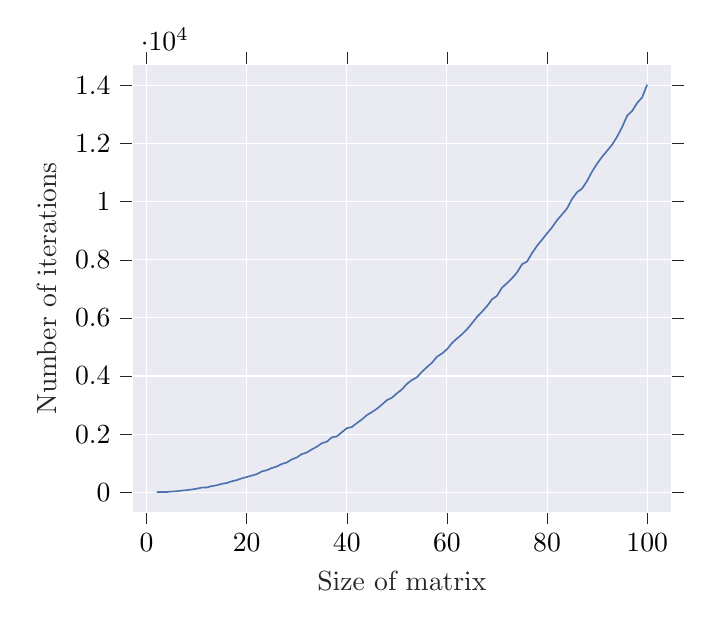
\begin{tikzpicture}

\definecolor{darkslategray38}{RGB}{38,38,38}
\definecolor{lavender234234242}{RGB}{234,234,242}
\definecolor{steelblue76114176}{RGB}{76,114,176}

\begin{axis}[
axis background/.style={fill=lavender234234242},
axis line style={white},
mark options={mark size=2.5pt, line width=1.5pt},
minor xtick={},
minor ytick={},
tick align=outside,
title style={align=center},
x grid style={white},
xlabel=\textcolor{darkslategray38}{Size of matrix},
xmajorgrids,
xmajorticks=false,
xmajorticks=true,
xmin=-2.9, xmax=104.9,
xtick style={color=darkslategray38},
xtick={-20,0,20,40,60,80,100,120},
y grid style={white},
ylabel=\textcolor{darkslategray38}{Number of iterations},
ymajorgrids,
ymajorticks=false,
ymajorticks=true,
ymin=-700.7, ymax=14736.7,
ytick style={color=darkslategray38},
ytick={-2000,0,2000,4000,6000,8000,10000,12000,14000,16000}
]
\addplot [semithick, steelblue76114176]
table {%
2 1
3 7
4 6
5 24
6 31
7 54
8 70
9 92
10 119
11 156
12 162
13 209
14 237
15 286
16 316
17 373
18 413
19 475
20 522
21 571
22 618
23 711
24 757
25 830
26 882
27 970
28 1021
29 1127
30 1195
31 1309
32 1366
33 1474
34 1564
35 1685
36 1738
37 1886
38 1919
39 2064
40 2201
41 2245
42 2378
43 2501
44 2654
45 2755
46 2869
47 3015
48 3167
49 3251
50 3403
51 3538
52 3726
53 3861
54 3957
55 4144
56 4304
57 4456
58 4662
59 4772
60 4919
61 5131
62 5291
63 5437
64 5605
65 5816
66 6033
67 6214
68 6405
69 6641
70 6761
71 7043
72 7196
73 7365
74 7565
75 7847
76 7942
77 8232
78 8484
79 8694
80 8913
81 9118
82 9367
83 9563
84 9770
85 10100
86 10327
87 10455
88 10716
89 11042
90 11312
91 11551
92 11754
93 11966
94 12243
95 12572
96 12962
97 13128
98 13401
99 13596
100 14035
};
\end{axis}

\end{tikzpicture}
